\documentclass{beamer}
\usepackage[T1]{fontenc}
\usepackage[utf8]{inputenc}

\usepackage{pgf,pgfpages}
\usepackage{tikz}
\usetikzlibrary{arrows,shapes,backgrounds,calc}

\usepackage{graphicx}
\usepackage{colortbl}
\usepackage{units}

%% Beamer style >>>>>>>>>>>>>>>>>>>>>>>>>
\mode<presentation>
{
  \usetheme{PHD}
  \setbeamercovered{transparent}
  \setbeamertemplate{items}[square]
}

%\usefonttheme[onlymath]{serif}

\beamertemplatenavigationsymbolsempty

\defbeamertemplate{enumerate item}{mycircle}
{
  %\usebeamerfont*{item projected}%
  \usebeamercolor[bg]{item projected}%
  \begin{pgfpicture}{0ex}{0ex}{1.5ex}{0ex}
    \pgfcircle[fill]{\pgfpoint{-0.1pt}{.65ex}}{1.1ex}
    \pgfbox[center,base]{\color{PHDyellow}{\insertenumlabel}}
  \end{pgfpicture}%
}
[action]
{\setbeamerfont{item projected}{size=\scriptsize}}
\setbeamertemplate{enumerate item}[mycircle]

%<<<<<<<<<<<<< beamer style

\title[Numerical Models Oceanography]{Analysis and Numerical Simulation of some Mathematical Models in Oceanography}
\author[J.R. Rodr\'{\i}guez Galv\'an]{J. Rafael Rodr\'{\i}guez Galv\'an}
\date{\today}

% XeLaTeX font choosing
% \usepackage{fontspec}%{xltxtra} %fontspec}
% \setsansfont{Fontin Sans}
% \setsansfont{Lato}

% PDFLaTeX font choosing
\usepackage[default, scale=1.0]{lato}

% Different math fonts, see http://tug.org/pracjourn/2006-1/hartke/hartke.pdf
%\usepackage{eulervm}
%\usepackage{ccfonts, eulervm}
%\usepackage[math]{kurier}
%\usepackage[math]{anttor}
%\usepackage{pxfonts}
%\usepackage{mathpazo}
%\usepackage{mathpple}
%\usepackage[varg]{txfonts}
%\usepackage{arev}
%\usepackage{fourier}

\usepackage{tabularx}
\usepackage{array, multirow, booktabs, rotating} % booktabs: toprule, midrule...

% Define a special style at begining of sections
\newcommand{\SetEmptyBackground}{
  \setbeamertemplate{background}{}
  \setbeamertemplate{footline}[default]
}
\newcommand{\SetDefaultBackground}{
  \setbeamertemplate{background}
  {
\includegraphics[width=\paperwidth,height=\paperheight]{slide_bg}}
  \setbeamertemplate{footline}[PHDtheme]
}
\newenvironment{sectionframe}{%
  \SetEmptyBackground\begin{frame}
%    \par\noindent\structure{\rule{\linewidth}{1pt}}\par
%    \vskip+0.6em
    \vskip1.6em
    Section \thesection.  \itshape\insertsection
    \vskip-0.7em
    \par\noindent\structure{\rule{\linewidth}{1pt}}\par
  }{%
  \end{frame}\SetDefaultBackground}

\newenvironment{smallblock}[1]{%
  % Block with horizontal top title
  \begin{block}{\small #1}
    \vspace{-0.9\baselineskip}
    \small
  }{\vspace{-1.2\baselineskip}\end{block}}

\newenvironment{smallblockTurn}[1]{%
  \begin{block}{}
    \vspace{-0.4\baselineskip}
    \small
    \begin{tabular}{@{}l|>{$}r<{$}>{$}l<{$}@{}}
      \multirow{3}{*}{
        \begin{turn}{40}
          #1
        \end{turn}}&
      \begin{minipage}{0.8\linewidth}
      }{\vspace{-1.0\baselineskip}%
      \end{minipage}\end{tabular}\end{block}}

\newenvironment{BlockNoTitle}{%
  \HideBlockTitle%
  \begin{block}{}}{%
  \end{block}%
  \ResetBlockTitle}

\newenvironment{BoxWithVerticalLabel}[2]{%
%  \begin{tabular}{@{\quad}r@{ }l@{}}
  \mbox{}\quad
  \begin{rotate}{90}
    \color{black}\small\fbox{#1}
  \end{rotate}}%&}
{}
%{\end{tabular}}

\newcommand{\heatProblem}{(Heat-Problem)\xspace}
\newcommand{\poissonProblem}{(Poisson-Problem)\xspace}

% % Video playing
% % Commands with two or more optional arguments
% % (see http://tex.stackexchange.com/questions/29973/more-than-one-optional-argument-for-newcommand)
% \usepackage{xparse} % From future LaTeX 3
% \DeclareDocumentCommand{\PlayVideoWithLabelAutostart}{%
%   O{0.5\linewidth} O{0.5\linewidth}  O{} m }{%
%   % #1: width of video box
%   % #2: height of video box
%   % #3: Label
%   % #4: Video file
%   \begin{BoxWithVerticalLabel}{#3}{#1}
%     \href{run:#4?autostart}{\rule{#1}{#2}}
%   \end{BoxWithVerticalLabel}}

% \DeclareDocumentCommand{\PlayVideoWithNoLabelAutostart}{%
%   O{0.5\linewidth} O{0.5\linewidth} m }{%
%   \href{run:#3?autostart}{\rule{#1}{#2}}}

% \DeclareDocumentCommand{\PlayVideoNOAutoStart}{%
%   O{0.5\linewidth} O{1.0} O{} m }{%
%   \href{run:#3}{\rule{#1}{#2}}}

% \DeclareDocumentCommand{\PlayVideoWithLabelNOAutostart}{%
%   O{0.5\linewidth} O{1.0} O{} m }{%
%   \begin{BoxWithVerticalLabel}{#3}{#1}
%     \href{run:#4}{\rule{#1}{#2}}
%   \end{BoxWithVerticalLabel}}

% \DeclareDocumentCommand{\PlayVideoWithLabel}{%
%   O{0.5\linewidth} O{1.0}  O{} m }{\PlayVideoWithLabelAutostart[#1][#2][#3]{#4}}

% % \DeclareDocumentCommand{\PlayVideoWithLabel}{%
% %   O{0.5\linewidth} O{1.0}  O{} m }{\PlayVideoWithLabelNOAutostart[#1][#2][#3]{#4}}

\usepackage{numerical-oceanography}

\newtheorem{remark}{Remark}
\newtheorem{proposition}{Proposition}
%\newtheorem{theorem}{Theorem}

% Presentation goodies >>>>>>>>>>>>>>>>>>>>>>>>>>>>
\newcommand<>{\myframed}[1]{\alt#2{\tikz[phd] \node[box] {#1};}{{#1}}}
\newcommand<>{\myframedAlert}[1]{\alt#2{\tikz[phdB] \node[boxB] {\color{black}#1};}{{#1}}}
\newcommand<>{\framedmath}[1]{%
\alt#2{\tikz[phd] \node[box] {\ensuremath{#1}};}{\ensuremath{#1}}}
\newcommand{\framedB}[1]{\tikz[phd] \node[boxB] {#1};}
\newcommand{\framedmathB}[1]{\framedB{\ensuremath{\displaystyle{#1}}}}
\newcommand{\ver}[1]{\footnote{See #1}}
\newcommand{\cita}[1]{{\color{PHDgray}\cite{#1}}}
\newcommand\cellalert[2]{\only<#1>{\cellcolor{PHDyellow}}\alt<#1>{\textbf{#2}}{#2}}
\newcommand{\soften}[1]{{\color{PHDgray}#1}}
\newcommand{\rowalert}[7]{%
    \cellalert{#1}{#2} & \cellalert{#1}{#3} &
    \cellalert{#1}{#4} & \cellalert{#1}{#5} &
    \cellalert{#1}{#6} & \cellalert{#1}{#7}}

\newcommand{\kk}{\Delta t}
% \usepackage{wasysym}
% \newcommand{\good}{{\color{PHDgreen}$\CIRCLE$}} %\blacksmiley
% \newcommand{\bad}{{\color{PHDred}$\CIRCLE$}}
\usepackage{pifont}
\newcommand{\good}{{\color{PHDgreen}\ding{52}}}
\newcommand{\bad}{{\color{PHDred}\ding{56}}}
\newcommand{\exclamation}{{\large\color{PHDred}{\textbf{\itshape !}}}}
\newcommand{\question}{{\large\color{PHDred}{\textbf{\itshape ?}}}}
\newcommand\colorUnderLine[2][PHDyellow]{\color{#1}\underline{{\color{black}#2}}\color{black}\xspace}
\newcommand\gris{\color{PHDgray}}
\newcommand\amarillo{\color{PHDyellow}}
\newcommand\tiragris[1]{{\par\hfill\small\gris{#1}}}
%<<<<<<<<<<<<<<<

\setcounter{tocdepth}{1}


%
% Bibliography
%
%\usepackage{natbib}

% To list each bibliographic entry in a line
\setbeamertemplate{bibliography entry title}{}
\setbeamertemplate{bibliography entry location}{}
\setbeamertemplate{bibliography entry note}{}

% \includeonly{
  % sec-intro,
  % sec-hydrstokes-stability,
  % sec-stokes,
  % sec-hydrstokes-tests,
  % sec-v-stabilized,
  % sec-vardens-time
 % }

%\includeonly{sec-stokes}
%\includeonly{sec-hydrstokes-tests}
% \includeonly{sec-v-stabilized}
%\includeonly{sec-vardens-time}

% ... end of preamble.

%======================================================================
\begin{document}
%======================================================================

% Tikz style and beamer template ------->>>
\tikzstyle{every picture}+=[remember picture]
\tikzstyle{na} = [baseline=-.5ex]
\tikzstyle{phd} = [baseline=-.6ex,
  box/.style={rectangle, draw=PHDblueC, thick, fill=PHDblueA,
    align=center, rounded corners, minimum height=1.6em},
  boxB/.style={rectangle, draw=PHDredA, thick, fill=PHDblueA,
    align=center, rounded corners, minimum height=1.6em}]
\tikzstyle{phdB} = [baseline=-.7ex,
  box/.style={rectangle, draw=PHDblueC, thick, fill=PHDblueA,
    align=center, rounded corners, minimum height=1.6em},
  boxB/.style={rectangle, draw=PHDredA, thick, fill=PHDblueA,
    align=center, rounded corners, minimum height=1.6em}]
\tikzstyle{myarrow} = [->,>=latex, PHDredA, shorten >=4pt,
  opacity=.6, line width=0.6mm]
\tikzstyle{myarrow2} = [->,>=latex, PHDblueC, shorten >=4pt, opacity=.2, line width=0.4mm]
\tikzstyle{myarrow3} = [
     opacity=.7,
%    >=triangle 60,              % Nice arrows; your taste may be different
    node distance=6mm and 60mm, % Global setup of box spacing
    every join/.style={norm},   % Default linetype for connecting
                                % boxes
    line width=0.6mm,
    PHDredA,
    ->
    ]
\setbeamertemplate{background}
 {
\includegraphics[width=\paperwidth,height=\paperheight]{frontpage_bg}}
\setbeamertemplate{footline}[default]
% <<<-------


% Write custom titlepage ------->>>
\begin{frame}
  \titlepage
  \vspace{5cm}
\end{frame}

% Set the background for the rest of the slides.
\setbeamertemplate{background}
 {
\includegraphics[width=\paperwidth,height=\paperheight]{slide_bg}}


% Write all of the slides..........

\begin{frame}{Outline}
  \tableofcontents
\end{frame}

% Start inserting infoline at the end
\setbeamertemplate{footline}[PHDtheme]
% <<<-------

\newcommand{\imgdir}{Undefined, use renewcommand!}

%%,---------------------------------------------------------------------
%%| Introduction
%%`---------------------------------------------------------------------
\section[Introduction]{Mathematical Modelling and Numerical Simulation}
\label{sec:introduction}
\begin{frame}{Mathematical Modelling and Numerical Simulation}
  \begin{itemize}
  \item \alert{Mathematical Model}: representation of physical reality
    that is suitable for \textit{analysis} and \textit{calculation}
  \item \alert{Numerical Simulation} allows us to \textit{calculate the
    solution of a model} in a computer and therefore to simulate
    physical reality
  \end{itemize}
  \medskip
  In this work\dots
  \smallskip
  \begin{itemize}
  \item models defined by \textbf{PDEs} (Partial Differential Equations)
  \item we shall introduce models of \textit{increasing complexity}
  \item targets:
    \begin{itemize}
    \item to explore and \textit{analyze} models in large-scale
      \textbf{Oceanography}
    \item to develop \textit{numerical methods} for simulate
      ocean flow
    \end{itemize}
  \end{itemize}
\end{frame}

\begin{frame}{A First Example of Modelling}
  Modelling requires \alert{great effort} for an applied mathematician
  \begin{itemize}
  \item Thorough knowledge of \llaveizq{\textit{mathematics}\\\textit{scientific discipline}}
  \item To communicate with other scientists, to select the adequate
    model between different possibilities, to simplify models which
    are too complex\dots
  \item In later stage, also \textit{computing skills}
  \end{itemize}

  \bigskip
  We start describing a simple model: the \alert{Heat Equation}
\end{frame}

\SetEmptyBackground
\begin{frame}
  Let
  \begin{itemize}
  \item $\Omega\subset\Rset^N$, \quad ($N=1,2,3$), \ open spatial domain \tiragris{occupied by a
      homogeneous, isotropic, heat conductor material}
  \item $\xx=(x_1,\dots,x_N) \in \Omega$: \textit{space} variable, \quad $t\in (0,T)$: \textit{time} variable
  \item \textit{Temperature}: unknown function,
    \begin{align*}
    u:\Omega\times (0,T) \to \Rset, \\
      (\xx,t) \mapsto u(\xx,t).
    \end{align*}
    \vspace{-1em}
    \pause
  \item \textit{Heat source}: a given function, $f(\xx,t)$
    \vspace{0.66em}
  \item Using physical laws (see e.g.~\cite{allaire:2007}),
    \begin{itemize}
    \item conservation of energy (of heat),
    \item quantity of heat is proportional to temperature: $c u$, \ $c\in\Rset$,
    \item heat flux proportional to temperature gradient: $q=-k\grad u$, $k\in\Rset$,
      \tiragris{\tiny $c$, $k$: physical
        constants (dependent on material), called ``specific heat'' and ``thermal conductivity''}
    \end{itemize}
  \item \dots and some mathematical theory (Gauss theorem), we arrive to\dots
  \end{itemize}
\end{frame}

\SetDefaultBackground
\begin{frame}{The Heat Equation}
  \begin{itemize}
  \item ... we arrive to the following \textbf{PDE} in $\Omega$:
    \begin{BlockNoTitle}
      \begin{equation*}
        c\, \framedmath<2>{\dt u} - k\, \framedmath<3>{\Delta u} = f
        \qquad \soften{\text{in} \quad \Omega\times (0,T),}
      \end{equation*}
    \end{BlockNoTitle}
    where:
    \begin{itemize}
    \item $\framedmath<2>{\dt u} = \frac{\partial u}{\partial t}$
      \quad (time partial derivative)
    \item
      $\framedmath<3>{\Delta u} = \sum_{i=1}^N \frac{\partial^2
        u}{\partial x_i^2}$ \quad (Laplacian operator)
    \end{itemize}
    \bigskip
    \item<4-> We must add an \textbf{initial condition}
      \soften{(state of the model at time $t=0$)}:
      \begin{BlockNoTitle}
        \begin{equation*}
          u(\xx,0) = u_0(\xx), \soften{ \qquad \forall \xx\in\Omega}
        \end{equation*}
      \end{BlockNoTitle}

    \item<4->
      And also \textbf{boundary conditions}
      \soften{(evolution of the model on the boundary,
        $\xx\in\partial\Omega$)}\dots
  \end{itemize}
\end{frame}

\begin{frame}{Boundary Conditions {\small (to select depending on physical context)}}
  % \vspace{-1.5em}
  % Different possibilities to select \soften{ (depending on physical context)}:
  % \medskip
  \begin{enumerate}
  \item \alert{Dirichlet} boundary condition:
    \begin{BlockNoTitle}
      \begin{equation*}
        u(\xx,t)=0, \quad \forall \xx\in\partial\Omega, \quad \forall t\in(0,T)
      \end{equation*}
    \end{BlockNoTitle}
  \item \alert{Neumman} boundary condition:
    \begin{BlockNoTitle}
      \begin{equation*}
        \partial_{\nn} u(\xx,t) := \grad u(\xx,t)\cdot\nn = 0,
      \end{equation*}
    \end{BlockNoTitle}
    {\small\hfill
     where $\grad u =$ gradient vector and $\nn=$ unit outward vector normal to $\Omega$.}
    \smallskip
    \tiragris{\scriptsize{}
        \textbf{Interpretation}: No heat flux across $\partial\Omega$ (domain isolated from the exterior)}
  \item \alert{Robin} (or Fourier) boundary condition
    \begin{BlockNoTitle}
      \begin{equation*}
        \partial_{\nn} u(\xx,t) + \alpha u(\xx,t) = 0,
      \end{equation*}
    \end{BlockNoTitle}
    {\small\hfill where $\alpha>0$ is a given constant}
    \tiragris{\scriptsize
      \begin{tabular}{r}
      \textbf{Interpretation}: Heat flux trough $\partial\Omega$ is proportional to
        the difference \\ of temperature between exterior and interior
      \end{tabular}
    }
  \end{enumerate}
\end{frame}

\begin{frame}{The Heat Equation}
  We can summarize in the following problem: find $u(\xx,t)$ such that
  \begin{BlockNoTitle}%
    \begin{tabular}[t]{l|>{$}l<{$}l}
       \rotatebox[origin=c]{40}{\small \heatProblem}
      &
        \begin{aligned}%
          \dt u - \nu\, \Delta u &= f
          \qquad \text{in} \ \Omega\times (0,T),
          \\\noalign{\smallskip}
          u|_{t=0} &= u_0
          \qquad \text{in}\ \Omega,
          \\\noalign{\smallskip}
          u&=0
          \qquad \text{on}\ \partial\Omega \times (0,T),
        \end{aligned}
    \end{tabular}
  \end{BlockNoTitle}
  where $\nu=k/c>0$ (viscosity coefficient) and we fixed Dirichlet B.C.
  \pause
  \small
  \begin{remark}
    This problem has a universal character and is applied to model \structure{many phenomena}:
    \begin{itemize}
    \item Heat propagation
    \item Diffusion of a density or concentration (of biological
      species, of pollution,\dots)
    \item In finance, value of an option to buy a stock
    \item \dots
    \end{itemize}
  \end{remark}
\end{frame}

\begin{frame}{The Poisson Problem}
  For certain choices of the source term, $f(x)$, Heat Equation reaches a
  \alert{\textbf{steady}} or (\textbf{stationary}) state, that is
  $$
  u(\xx,t) \longrightarrow u_\infty(\xx) \quad\mbox{as}\quad t\to\infty.
  $$
  Often it is interesting to calculate the steady state directly, solving:
  \begin{BlockNoTitle}%
    \begin{tabular}[t]{l|>{$}l<{$}l}
       \rotatebox[origin=c]{30}{\small \poissonProblem}
      &
        \begin{aligned}%
          \Delta u &= f
          \qquad \text{in} \ \Omega,
          \\\noalign{\smallskip}
          u&=0
          \qquad \text{on}\ \partial\Omega.
        \end{aligned}
    \end{tabular}
  \end{BlockNoTitle}
  \medskip
  \pause
  Now we are about to use this simpler problem as example for:
  \smallskip
  \begin{enumerate}
  \item \emph{Analysis} of the model (including existence and uniqueness of solution) and
  \item \emph{Numerical simulation} (calculating the solution).
\end{enumerate}
\end{frame}

\begin{frame}{Variational Formulation of \poissonProblem}
  \small
  \begin{proposition}
  Let
  $$
  X=\{ \Phi\in C^1(\overline\Omega) \st \Phi=0 \quad \mbox{on } \partial\Omega\}.
  $$
  A function $u\in C^2(\Omega)$ is a solution of \poissonProblem $\mathbf\Longleftrightarrow$ $u\in X$ and satisfies:
  \begin{equation}
    \tag{\ensuremath{P_V}}
    \int_\Omega \grad u(\xx) \grad v(\xx) d\xx = \int_\Omega f(\xx) v(\xx) d\xx \quad \forall v\in X.
    \label{eq:poisson.variational}
  \end{equation}
  \end{proposition}
  \begin{itemize}
  \item Proof: follows from Green's formula (integration by parts).
  \item Problem (\ref{eq:poisson.variational}) is called
    \alert{\textbf{Variational Formulation}} of \poissonProblem.
  \item $v$ is called \textbf{test function}.
  \item (\ref{eq:poisson.variational}) only requires
    $u\in C^1(\Omega)$. In this sense it is \textbf{weaker} than ``classical
    formulation'' of \poissonProblem, which requires $u\in C^2(\Omega)$.
  \item $\Rightarrow$ we suspect that it is \textbf{easier to solve}
    (\ref{eq:poisson.variational}) than ``classical formulation''.
  \end{itemize}
  \vspace{-1em}
  \begin{BlockNoTitle}
    \begin{center}
      \textbf{Idea:} Is possible to develop a theory for
      well-posedness of~(\ref{eq:poisson.variational})? \ \dots
    \end{center}
  \end{BlockNoTitle}
\end{frame}

\begin{frame}{Abstract framework}
  \begin{itemize}
  \item Reformulation of (\ref{eq:poisson.variational}): find
    $u\in X$ such that
    \begin{BlockNoTitle}
      \begin{equation}
        \tag{\ensuremath{P_V}}
        a(u,v) = L(v) \quad \forall v\in
        X,\label{eq:abstract.variational}
      \end{equation}
    \end{BlockNoTitle}
    were $a(\cdot,\cdot)$ and $L(\cdot)$ \soften{are the following} bilinear and linear forms:
    \begin{equation*}
      a(u,v) = \int_\Omega \grad u \grad v, \qquad
      L(v) = \int_\Omega f  v.
    \end{equation*}

  \item There \alert{\textbf{exists a powerful theory}}
    (\structure{Lax-Milgram}) for analysing abstract variational
    formulations like~(\ref{eq:abstract.variational}).

  \item \soften{However, this theory} \textbf{only works for Hilbert spaces}. \soften{And}
    $$
    X=\{ \Phi\in C^1(\overline\Omega) \st \Phi=0 \quad \mbox{on } \partial\Omega\}
    $$
    is \textbf{not a Hilbert space} \soften{(equipped with  the "natural" scalar product for this problem)}.
  \item \soften{We therefore must} \alert{\textbf{replace $X$ with a Hilbert space}, $V$}.
  \end{itemize}
\end{frame}

\begin{frame}{Lax-Milgram Theory}
  \small
  Let $V$ a Hilbert space.
  \soften{Consider the abstract problem:}
  Find $u\in V$ such that
    \begin{BlockNoTitle}
      \begin{equation}
        \tag{\ensuremath{P_V}}
        a(u,v) = L(v) \quad \forall v\in V,
        \label{eq:abstract.variational.hilbert}
      \end{equation}
    \end{BlockNoTitle}
    \soften{and the following} hypothesis:
    \begin{enumerate}
    \item $L(\cdot)$ is \textbf{linear} and \textbf{continuous}, \soften{i.e.} $\exists C>0$ \soften{such that:}
      \label{item:1}
      \begin{equation*}
        |L(v)|\le C \norm[]{v} \quad \forall v\in V.
      \end{equation*}
    \item $a(\cdot,\cdot)$ is \textbf{bilinear} and \textbf{continuous}, \soften{i.e.} $\exists M>0$ \soften{such that:}
      \label{item:2}
      \begin{equation*}
        |a(v,w)|\le M \norm[]{v}\norm[]{w} \quad\forall v,w\in V,
      \end{equation*}
    \item $a(\cdot,\cdot)$ is \textbf{coercive}, \soften{i.e.} $\exists \nu>0$ \soften{such that:}
      \label{item:3}
      \begin{equation*}
        |a(v,v)| \ge \nu  \norm[]{v}^2 \quad\forall v\in V,
      \end{equation*}
    \end{enumerate}
    \begin{theorem}[Lax-Milgram]
      Under previous
      hypothesis,~\alert{(\ref{eq:abstract.variational.hilbert})} is
        well posed, i.e., it \alert{\textbf{has a unique solution}} which
      depends continuously on $L$.
    \end{theorem}
\end{frame}

\begin{frame}{Sobolev spaces}
  \small
  \soften{Some results from \textbf{functional analysis}:}
  \begin{itemize}
  \setlength\itemsep{0.5em}
  \item<1->
    $L^p(\Omega)=\{ f: \Omega \to \Rset \quad \text{measurable} \st
    \alert{\int_\Omega |f(\xx)|^p < +\infty} \} \quad p \in [1,+\infty)$
    \begin{itemize}
      \setlength\itemsep{0.3em}
      \scriptsize
    \item $L^p(\Omega)$ is a Banach space for
      $\norm[L^p(\Omega)]{f}=\left(\int_\Omega|f(\xx)|^p\right)^{1/p}$
    \item $L^2(\Omega)$ is a Hilbert space for $(f,g)_{L^2(\Omega)}=\int_\Omega f(\xx) g(\xx) d\xx$
    \end{itemize}

  \item<2->
    $ H^m(\Omega) = \{ f\in L^2(\Omega) \st \text{\alert{weak derivatives} of
      order $|\alpha| \le m$ are \alert{in} } \alert{L^2(\Omega)} \} $
    \begin{itemize}
      \setlength\itemsep{0.3em}
      \scriptsize
    \item Hilbert space for
      $(f,g)_{H^m(\Omega)}=\sum_{|\alpha|\le m} \int_\Omega D^\alpha f
      \; D^\alpha g \,d\xx$.
      \par \soften{ which induces the norm:} \quad
      $\norm[H^m(\Omega)]{f}=\left(\sum_{|\alpha|\le m} \int_\Omega|D^\alpha f(\xx)|^2\right)^{1/2}$
      \item $C^\infty(\overline\Omega) \subset H^m(\Omega)$, dense inclusion.
    \end{itemize}

  \item<3-> \alert{$H_0^1(\Omega) = \{ v \in H^1(\Omega) \st v|_{\partial\Omega}=0 \}$}
     \hfill\soften{ (sense of $v|_{\partial\Omega}=0$ ? Trace theory)}
    \begin{itemize}
      \setlength\itemsep{0.3em}
      \scriptsize
    \item Hilbert space for
      $(f,g)_{H_0^1(\Omega)}=\int_\Omega \grad f \; \grad g \, d\xx $
      \par \soften{ which induces the norm:} \quad
      $\norm[H_0^1(\Omega)]{f}=\left(\int_\Omega|\grad f|^2\, d\xx\right)^{1/2}$
    \item $D(\Omega) =\{ \small \Phi\in C^\infty(\Omega) \st \text{ soporte compacto} \}
      \subset H_0^1(\Omega)$, dense.
       \small
     $$\Rightarrow
      D(\Omega) \subset \alert{X=\{ \Phi\in C^1(\overline\Omega) \st \Phi=0 \quad \mbox{on
      } \partial\Omega\} \subset H_0^1(\Omega)} \text{, dense}.$$
    \end{itemize}
  \end{itemize}
\end{frame}

\begin{frame}{Well-posedness of the Poisson Problem}
  \begin{theorem}
    Let $\Omega \subset \Rset^N$ open, bounded set. Take $f\in L^2(\Omega)$.
    \begin{enumerate}
    \item \alert{$\exists! u \in V=H_0^1(\Omega)$ solution} of the variational formulation
      \begin{equation}
        \tag{\ensuremath{P_V}}
        \int_\Omega \grad u \, \grad v \,d\xx = \int_\Omega f\, v \, d\xx \quad \forall v\in V.
        \label{eq:1}
      \end{equation}
    \item Further, it \alert{depends continuously on the data}, i.e., $\exists C>0$ such that
      $$
      \norm[H_0^1(\Omega)]{u} \le C \norm[L^2(\Omega)]{f}.
      $$
    \item If $\Omega$ is an open set of class $C^{m+2}$ and
      $f\in H^m(\Omega)$ with $m>N/2$, then the solution $u$
      of~(\ref{eq:1}) is a \alert{\textbf{strong} or \textbf{classical solution}} i.e. it verfies
      $$
      u\in C^2(\overline\Omega), \qquad -\Delta u(\xx) = f(\xx) \quad \forall \xx\in\Omega, \quad u|_{\partial\Omega}=0.
      $$
    \end{enumerate}
  \end{theorem}
  \scriptsize \textbf{Proof}: (1) and (2) are consequence of
  \structure{\textbf{Lax-Milgram}} Theorem. (3) requires more \structure{functional
    analysis}, see e.g.~\cite{brezis:2017,allaire:2007}.
\end{frame}

\begin{frame}{Numerical Simulation of the Poisson Problem}

\small
Construction of any numerical method for solving a (steady) PDE requires to consider:
\begin{enumerate}
\item How to represent the solution $u(\xx,t)$ by an
  \textit{approximate solution} $u_h(\xx,t)$?
\item In which sense the approximate solution $u_h (\xx,t)$
  satisfies the PDE?
\end{enumerate}

\bigskip

\textbf{Example}: \alert{\textbf{Finite Difference}} method for the \alert{Poisson
problem} (steady) in $\Omega=(0,1)\times (0,1) \subset\Rset^2$ \soften{(the unit
square)}:

\begin{enumerate}
\item We consider the mesh \structure{$\overline \Omega_h = \{ (x_i,y_j)=(ih,jh) \st 0 \le i,j \le M \} $}
and define $u_h(\xx)$ by piecewise interpolation of the approximations \structure{$u^h_{ij}\simeq u(x_i,y_j)$}
\item Partial derivatives are approximated \structure{on each node $(x_i,y_j)$} as incremental quotients:
  \begin{BlockNoTitle}
    \vspace{-1.5em}
    \begin{multline*}
      -\Delta u(x_i,y_j) = -\partial^2_{xx}u(x_i,y_j)
      -\partial^2_{yy}u(x_i,y_j)\simeq
      \\
      -\frac{u_{i-1,j}-2u_{ij}+u_{i+1,j}}{h^2}
      -\frac{u_{i,j-1}-2u_{ij}+u_{i,j+1}}{h^2} = f(x_i,x_j).
    \end{multline*}
  \end{BlockNoTitle}
  + B.C. $\Rightarrow$ \textbf{linear equations system}, $(M-1)^2$ equations and unknowns.
\end{enumerate}

\end{frame}

\begin{frame}{Finite Element Method}
  \small
  \begin{enumerate}
  \item We approximate $\overline\Omega$ by a \alert{triangulation
    ${\cal T}_h= \{K_i\}_{i}^M$}. Then select a \alert{polynomial order,
    $k\in\Nset$}, and define a finite-dimensional space
    \begin{BlockNoTitle}
      \vspace{-0.5em}
      $$
      V_h = \big\{ v_h\in C^0(\overline\Omega) \;\st\;
      v_h|_{K_i}\in\mathbb{P}_k, \ \forall K_i \in {\cal T}, \quad
      v_h|_{\partial\Omega}=0 \big\} \subset H_0^1(\Omega)
      $$
    \end{BlockNoTitle}
    This kind of approximations shall also be denoted as \alert{\P{k}}.
    \par \vspace{-0.7em}
    \setlength{\tabcolsep}{1.5em}
    \begin{center}
      \begin{tabular}{cc}
        \centering
        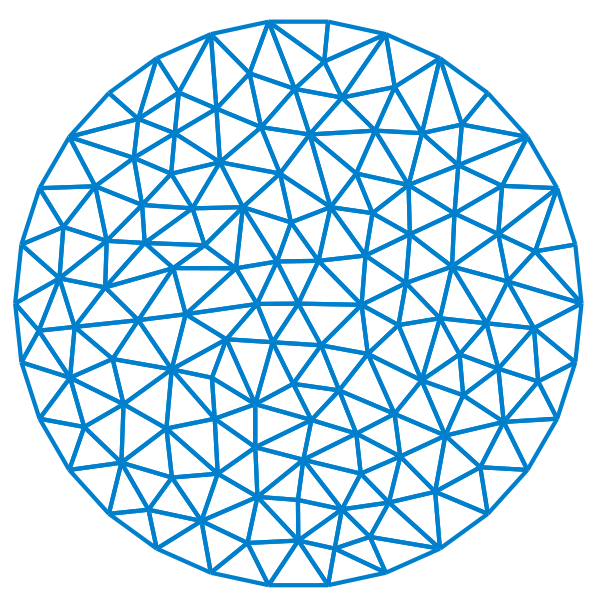
\includegraphics[height=0.20\linewidth]{img/FE_triangulation}
        &
          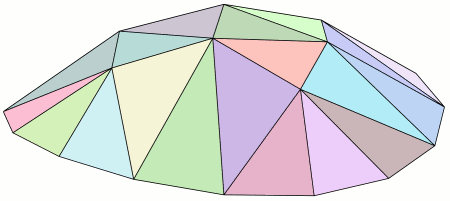
\includegraphics[height=0.15\linewidth]{img/FE_function_3d}
        \\
        {\scriptsize  Triangulation of $\overline\Omega$}
        &
          {\scriptsize Function $u_h \in V_h$ (\P1 approximation)}
      \end{tabular}
    \end{center}

  \item We \alert{approximate the \textbf{variational formulation}} of
    the Poisson problem as follows: find $u_h\in V_h$ such that:
    \begin{BlockNoTitle}
      \vspace{-0.5em}
      \begin{equation*}
        \int_\Omega \grad u_h(\xx) \grad v_h(\xx) d\xx = \int_\Omega f(\xx) v_h(\xx) d\xx \quad \forall v_h\in V_h.
        \label{eq:poisson.variational}
      \end{equation*}
    \end{BlockNoTitle}
  \end{enumerate}
\end{frame}

\begin{frame}
  \begin{theorem}
    Let ${\cal T}_h$ ($h\to 0$) be a sequence of regular meshes of
    $\Omega$. Let $u\in H_0^1(\Omega)$ be the solution of the Poisson
    problem and $u_h\in V_h$ its $\P{k}$ FE approximation. Then
    $$
    \lim_{h\to 0} \norm[H^1(\Omega)]{u-u_h} = 0.
    $$
    Moreover, if $u\in H^{k+1}$ and $k+1>N/2$, then we have the error estimate:
    $$
    \norm[H^1(\Omega)]{u-u_h} \le C \, h^k \, \norm[H^{k+1}(\Omega)]{u}.
    $$
    where $C$ is a constant (independent of $h$ and $u$).
  \end{theorem}
\end{frame}

%%% Local Variables:
%%% coding: utf-8
%%% TeX-master: "numerical-oceanography"
%%% mode: latex
%%% ispell-local-dictionary: "english"
%%% End:


% %%,---------------------------------------------------------------------
% %%| Hydrostatic Stokes Stability
% %%`---------------------------------------------------------------------
% \section{Hydrostatic Stokes Stability}
% \include{sec-hydrstokes-stability}

% %%,---------------------------------------------------------------------
% %%| Stokes with Unequal FE for Velocity
% %%`---------------------------------------------------------------------
% \section{Stokes with Unequal FE for Velocity}

%%,---------------------------------------------------------------------
%%| Hydrostatic Stable FE combinations}
%%`---------------------------------------------------------------------
\section{Hydrostatic Stable FE Combinations}
\label{sec:hydr-stable-fe}
% \include{sec-hydrstokes-stability}
% \include{sec-stokes}
% \include{sec-hydrstokes-tests}

%%,---------------------------------------------------------------------
%%|
%%`---------------------------------------------------------------------
\section{Stabilized Reformulations of Hydrostatic Stokes}
\label{sec:stab-reform-hydr}
% \include{sec-v-stabilized}

%%,---------------------------------------------------------------------
%%| Time schemes and variable denisity
%%`---------------------------------------------------------------------
\section{Time integration of the whole set of equations}
\label{sec:time-integr-whole}
% \include{sec-vardens-time}


%%,---------------------------------------------------------------------
%%| Conclusions and future work
%%`---------------------------------------------------------------------
\begin{frame}{Conclusions}
  \begin{itemize}\itemsep0.66em
  \item<1-> We have developed \alert{new schemes} for approximation of
    Primitive Equations of the Ocean (or even Anisotropic Navier-Stokes)
    \begin{itemize}
    \item Avoiding velocity instabilities of (quasi-)hydrostatic
      formulations
    \end{itemize}
  \item<2-> \alert{Standard FE tools and techniques} like mesh adaptation
    can be used, in \alert{more general meshes} than previous schemes
  \item<3-> Two different approached have been followed:
    \begin{itemize}
    \item New \alert{stable combinations of FE} (unequal
      approximation of velocity components)
    \item Reformulation of space schemes, \alert{stabilizing vertical
      velocity}. Hence standard Stokes--stable FE can be applied
    \end{itemize}
  \item<4-> Successfully applied to \alert{time-dependent problems},
    including \alert{variable density} and \alert{new time splitting}
    schemes
  \end{itemize}
  \uncover<5>{
  \begin{center}\it
    {In short, we have successfully introduced \textbf{a new approach}\\
    for modelling \textbf{realistic hydrostatic and quasi-hydrostatic fluids},\\
    justifying it both \textbf{analytically and numerically}.
  }
\end{center}
}

\end{frame}
\begin{frame}{~}
  \bigskip
  \Large Thank you for your attention.
  \vfill~
  \begin{flushright}
    \pgfsetfillopacity{0.4}
    \pgfimage[width=0.9\textwidth]{img/gibraltar-velocity-2d-difumin}
  \end{flushright}
\end{frame}

%%,-------------
%%| Bibliography
%%`-------------

\setbeamertemplate{footline}[default]

\begin{frame}[allowframebreaks]{Bibliography}
\bibliographystyle{alpha}
%\bibliographystyle{abbrvnat}
\bibliography{biblio-short.bib}
\end{frame}

\end{document}


%%% Local Variables:
%%% coding: utf-8
%%% TeX-master: t
%%% mode: latex
%%% ispell-local-dictionary: "english"
%%% End:
